\documentclass[1p]{elsarticle_modified}
%\bibliographystyle{elsarticle-num}

%\usepackage[colorlinks]{hyperref}
%\usepackage{abbrmath_seonhwa} %\Abb, \Ascr, \Acal ,\Abf, \Afrak
\usepackage{amsfonts}
\usepackage{amssymb}
\usepackage{amsmath}
\usepackage{amsthm}
\usepackage{scalefnt}
\usepackage{amsbsy}
\usepackage{kotex}
\usepackage{caption}
\usepackage{subfig}
\usepackage{color}
\usepackage{graphicx}
\usepackage{xcolor} %% white, black, red, green, blue, cyan, magenta, yellow
\usepackage{float}
\usepackage{setspace}
\usepackage{hyperref}

\usepackage{tikz}
\usetikzlibrary{arrows}

\usepackage{multirow}
\usepackage{array} % fixed length table
\usepackage{hhline}

%%%%%%%%%%%%%%%%%%%%%
\makeatletter
\renewcommand*\env@matrix[1][\arraystretch]{%
	\edef\arraystretch{#1}%
	\hskip -\arraycolsep
	\let\@ifnextchar\new@ifnextchar
	\array{*\c@MaxMatrixCols c}}
\makeatother %https://tex.stackexchange.com/questions/14071/how-can-i-increase-the-line-spacing-in-a-matrix
%%%%%%%%%%%%%%%

\usepackage[normalem]{ulem}

\newcommand{\msout}[1]{\ifmmode\text{\sout{\ensuremath{#1}}}\else\sout{#1}\fi}
%SOURCE: \msout is \stkout macro in https://tex.stackexchange.com/questions/20609/strikeout-in-math-mode

\newcommand{\cancel}[1]{
	\ifmmode
	{\color{red}\msout{#1}}
	\else
	{\color{red}\sout{#1}}
	\fi
}

\newcommand{\add}[1]{
	{\color{blue}\uwave{#1}}
}

\newcommand{\replace}[2]{
	\ifmmode
	{\color{red}\msout{#1}}{\color{blue}\uwave{#2}}
	\else
	{\color{red}\sout{#1}}{\color{blue}\uwave{#2}}
	\fi
}

\newcommand{\Sol}{\mathcal{S}} %segment
\newcommand{\D}{D} %diagram
\newcommand{\A}{\mathcal{A}} %arc


%%%%%%%%%%%%%%%%%%%%%%%%%%%%%5 test

\def\sl{\operatorname{\textup{SL}}(2,\Cbb)}
\def\psl{\operatorname{\textup{PSL}}(2,\Cbb)}
\def\quan{\mkern 1mu \triangleright \mkern 1mu}

\theoremstyle{definition}
\newtheorem{thm}{Theorem}[section]
\newtheorem{prop}[thm]{Proposition}
\newtheorem{lem}[thm]{Lemma}
\newtheorem{ques}[thm]{Question}
\newtheorem{cor}[thm]{Corollary}
\newtheorem{defn}[thm]{Definition}
\newtheorem{exam}[thm]{Example}
\newtheorem{rmk}[thm]{Remark}
\newtheorem{alg}[thm]{Algorithm}

\newcommand{\I}{\sqrt{-1}}
\begin{document}

%\begin{frontmatter}
%
%\title{Boundary parabolic representations of knots up to 8 crossings}
%
%%% Group authors per affiliation:
%\author{Yunhi Cho} 
%\address{Department of Mathematics, University of Seoul, Seoul, Korea}
%\ead{yhcho@uos.ac.kr}
%
%
%\author{Seonhwa Kim} %\fnref{s_kim}}
%\address{Center for Geometry and Physics, Institute for Basic Science, Pohang, 37673, Korea}
%\ead{ryeona17@ibs.re.kr}
%
%\author{Hyuk Kim}
%\address{Department of Mathematical Sciences, Seoul National University, Seoul 08826, Korea}
%\ead{hyukkim@snu.ac.kr}
%
%\author{Seokbeom Yoon}
%\address{Department of Mathematical Sciences, Seoul National University, Seoul, 08826,  Korea}
%\ead{sbyoon15@snu.ac.kr}
%
%\begin{abstract}
%We find all boundary parabolic representation of knots up to 8 crossings.
%
%\end{abstract}
%\begin{keyword}
%    \MSC[2010] 57M25 
%\end{keyword}
%
%\end{frontmatter}

%\linenumbers
%\tableofcontents
%
\newcommand\colored[1]{\textcolor{white}{\rule[-0.35ex]{0.8em}{1.4ex}}\kern-0.8em\color{red} #1}%
%\newcommand\colored[1]{\textcolor{white}{ #1}\kern-2.17ex	\textcolor{white}{ #1}\kern-1.81ex	\textcolor{white}{ #1}\kern-2.15ex\color{red}#1	}

{\Large $\underline{12n_{0052}~(K12n_{0052})}$}

\setlength{\tabcolsep}{10pt}
\renewcommand{\arraystretch}{1.6}
\vspace{1cm}\begin{tabular}{m{100pt}>{\centering\arraybackslash}m{274pt}}
\multirow{5}{120pt}{
	\centering
	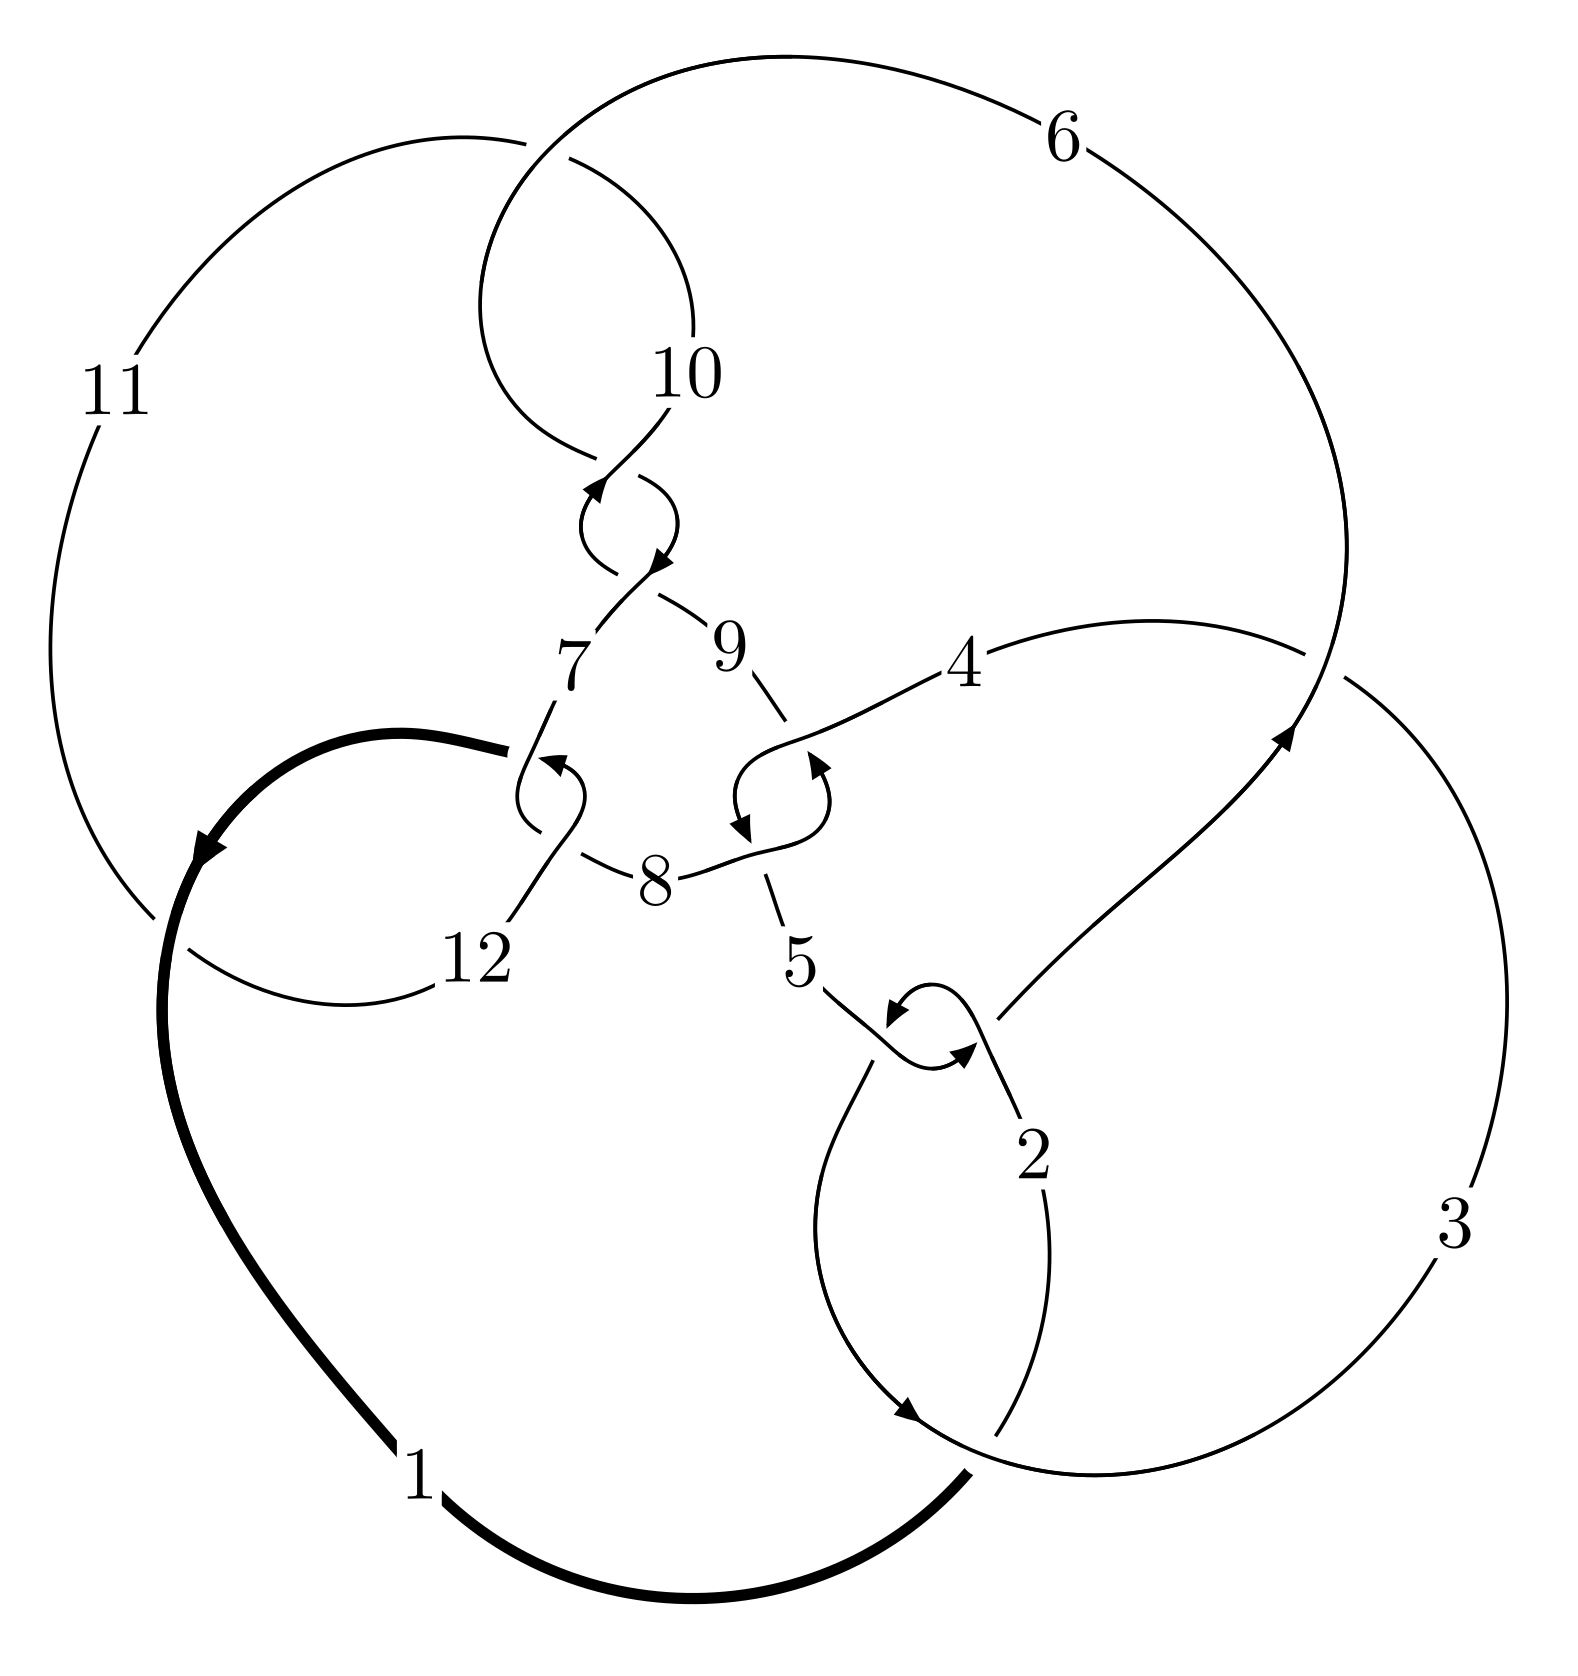
\includegraphics[width=112pt]{../../../GIT/diagram.site/Diagrams/png/2141_12n_0052.png}\\
\ \ \ A knot diagram\footnotemark}&
\allowdisplaybreaks
\textbf{Linearized knot diagam} \\
\cline{2-2}
 &
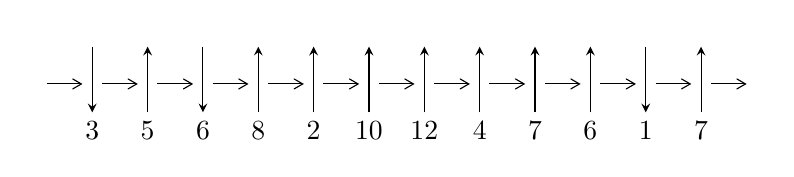
\begin{tikzpicture}[x=20pt, y=17pt]
	% nodes
	\node (C0) at (0, 0) {};
	\node (C1) at (1, 0) {};
	\node (C1U) at (1, +1) {};
	\node (C1D) at (1, -1) {3};

	\node (C2) at (2, 0) {};
	\node (C2U) at (2, +1) {};
	\node (C2D) at (2, -1) {5};

	\node (C3) at (3, 0) {};
	\node (C3U) at (3, +1) {};
	\node (C3D) at (3, -1) {6};

	\node (C4) at (4, 0) {};
	\node (C4U) at (4, +1) {};
	\node (C4D) at (4, -1) {8};

	\node (C5) at (5, 0) {};
	\node (C5U) at (5, +1) {};
	\node (C5D) at (5, -1) {2};

	\node (C6) at (6, 0) {};
	\node (C6U) at (6, +1) {};
	\node (C6D) at (6, -1) {10};

	\node (C7) at (7, 0) {};
	\node (C7U) at (7, +1) {};
	\node (C7D) at (7, -1) {12};

	\node (C8) at (8, 0) {};
	\node (C8U) at (8, +1) {};
	\node (C8D) at (8, -1) {4};

	\node (C9) at (9, 0) {};
	\node (C9U) at (9, +1) {};
	\node (C9D) at (9, -1) {7};

	\node (C10) at (10, 0) {};
	\node (C10U) at (10, +1) {};
	\node (C10D) at (10, -1) {6};

	\node (C11) at (11, 0) {};
	\node (C11U) at (11, +1) {};
	\node (C11D) at (11, -1) {1};

	\node (C12) at (12, 0) {};
	\node (C12U) at (12, +1) {};
	\node (C12D) at (12, -1) {7};
	\node (C13) at (13, 0) {};

	% arrows
	\draw[->,>={angle 60}]
	(C0) edge (C1) (C1) edge (C2) (C2) edge (C3) (C3) edge (C4) (C4) edge (C5) (C5) edge (C6) (C6) edge (C7) (C7) edge (C8) (C8) edge (C9) (C9) edge (C10) (C10) edge (C11) (C11) edge (C12) (C12) edge (C13) ;	\draw[->,>=stealth]
	(C1U) edge (C1D) (C2D) edge (C2U) (C3U) edge (C3D) (C4D) edge (C4U) (C5D) edge (C5U) (C6D) edge (C6U) (C7D) edge (C7U) (C8D) edge (C8U) (C9D) edge (C9U) (C10D) edge (C10U) (C11U) edge (C11D) (C12D) edge (C12U) ;
	\end{tikzpicture} \\
\hhline{~~} \\& 
\textbf{Solving Sequence} \\ \cline{2-2} 
 &
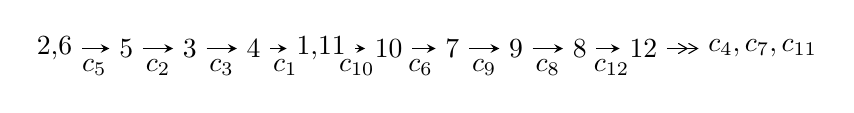
\begin{tikzpicture}[x=23pt, y=7pt]
	% node
	\node (A0) at (-1/8, 0) {2,6};
	\node (A1) at (1, 0) {5};
	\node (A2) at (2, 0) {3};
	\node (A3) at (3, 0) {4};
	\node (A4) at (65/16, 0) {1,11};
	\node (A5) at (41/8, 0) {10};
	\node (A6) at (49/8, 0) {7};
	\node (A7) at (57/8, 0) {9};
	\node (A8) at (65/8, 0) {8};
	\node (A9) at (73/8, 0) {12};
	\node (C1) at (1/2, -1) {$c_{5}$};
	\node (C2) at (3/2, -1) {$c_{2}$};
	\node (C3) at (5/2, -1) {$c_{3}$};
	\node (C4) at (7/2, -1) {$c_{1}$};
	\node (C5) at (37/8, -1) {$c_{10}$};
	\node (C6) at (45/8, -1) {$c_{6}$};
	\node (C7) at (53/8, -1) {$c_{9}$};
	\node (C8) at (61/8, -1) {$c_{8}$};
	\node (C9) at (69/8, -1) {$c_{12}$};
	\node (A10) at (11, 0) {$c_{4},c_{7},c_{11}$};

	% edge
	\draw[->,>=stealth]	
	(A0) edge (A1) (A1) edge (A2) (A2) edge (A3) (A3) edge (A4) (A4) edge (A5) (A5) edge (A6) (A6) edge (A7) (A7) edge (A8) (A8) edge (A9) ;
	\draw[->>,>={angle 60}]	
	(A9) edge (A10);
\end{tikzpicture} \\ 

\end{tabular} \\

\footnotetext{
The image of knot diagram is generated by the software ``\textbf{Draw programme}" developed by Andrew Bartholomew(\url{http://www.layer8.co.uk/maths/draw/index.htm\#Running-draw}), where we modified some parts for our purpose(\url{https://github.com/CATsTAILs/LinksPainter}).
}\phantom \\ \newline 
\centering \textbf{Ideals for irreducible components\footnotemark of $X_{\text{par}}$} 
 
\begin{align*}
I^u_{1}&=\langle 
-31828697846 u^{32}+114828956540 u^{31}+\cdots+560421961026 b+532030527306,\\
\phantom{I^u_{1}}&\phantom{= \langle  }-197273519317 u^{32}+385887384126 u^{31}+\cdots+1120843922052 a+266870259643,\\
\phantom{I^u_{1}}&\phantom{= \langle  }u^{33}-2 u^{32}+\cdots+5 u+4\rangle \\
I^u_{2}&=\langle 
- u^{19} a+2 u^{19}+\cdots+2 a+1,\;-2 u^{19}+3 u^{18}+\cdots-4 a+3,\;u^{20}- u^{19}+\cdots-2 u+1\rangle \\
I^u_{3}&=\langle 
- u^4 a-2 u^2 a+u^3+a u+b- a+u-1,\;2 u^4 a+4 u^3 a+6 u^2 a-3 u^3+a^2+4 a u-5 u^2+2 a-8 u-4,\\
\phantom{I^u_{3}}&\phantom{= \langle  }u^5+u^4+2 u^3+u^2+u+1\rangle \\
I^u_{4}&=\langle 
b+1,\;2 a-2 u+3,\;u^2- u+1\rangle \\
\\
\end{align*}
\raggedright * 4 irreducible components of $\dim_{\mathbb{C}}=0$, with total 85 representations.\\
\footnotetext{All coefficients of polynomials are rational numbers. But the coefficients are sometimes approximated in decimal forms when there is not enough margin.}
\newpage
\renewcommand{\arraystretch}{1}
\centering \section*{I. $I^u_{1}= \langle -3.18\times10^{10} u^{32}+1.15\times10^{11} u^{31}+\cdots+5.60\times10^{11} b+5.32\times10^{11},\;-1.97\times10^{11} u^{32}+3.86\times10^{11} u^{31}+\cdots+1.12\times10^{12} a+2.67\times10^{11},\;u^{33}-2 u^{32}+\cdots+5 u+4 \rangle$}
\flushleft \textbf{(i) Arc colorings}\\
\begin{tabular}{m{7pt} m{180pt} m{7pt} m{180pt} }
\flushright $a_{2}=$&$\begin{pmatrix}0\\u\end{pmatrix}$ \\
\flushright $a_{6}=$&$\begin{pmatrix}1\\0\end{pmatrix}$ \\
\flushright $a_{5}=$&$\begin{pmatrix}1\\u^2\end{pmatrix}$ \\
\flushright $a_{3}=$&$\begin{pmatrix}u\\u^3+u\end{pmatrix}$ \\
\flushright $a_{4}=$&$\begin{pmatrix}- u^3\\u^3+u\end{pmatrix}$ \\
\flushright $a_{1}=$&$\begin{pmatrix}u^3\\u^5+u^3+u\end{pmatrix}$ \\
\flushright $a_{11}=$&$\begin{pmatrix}0.176004 u^{32}-0.344283 u^{31}+\cdots-1.32385 u-0.238098\\0.0567942 u^{32}-0.204897 u^{31}+\cdots-0.869757 u-0.949339\end{pmatrix}$ \\
\flushright $a_{10}=$&$\begin{pmatrix}0.119210 u^{32}-0.139386 u^{31}+\cdots-0.454097 u+0.711242\\0.0567942 u^{32}-0.204897 u^{31}+\cdots-0.869757 u-0.949339\end{pmatrix}$ \\
\flushright $a_{7}=$&$\begin{pmatrix}0.207329 u^{32}-0.154336 u^{31}+\cdots-0.127694 u+1.18034\\0.00997898 u^{32}-0.246238 u^{31}+\cdots-1.25132 u-0.881877\end{pmatrix}$ \\
\flushright $a_{9}=$&$\begin{pmatrix}0.322990 u^{32}-0.306718 u^{31}+\cdots+0.284165 u+1.39874\\0.0620557 u^{32}-0.436306 u^{31}+\cdots-2.88278 u-1.94300\end{pmatrix}$ \\
\flushright $a_{8}=$&$\begin{pmatrix}0.442680 u^{32}-0.385581 u^{31}+\cdots+0.406459 u+1.30251\\0.00301080 u^{32}-0.502789 u^{31}+\cdots-2.70870 u-1.78276\end{pmatrix}$ \\
\flushright $a_{12}=$&$\begin{pmatrix}0.203780 u^{32}-0.167332 u^{31}+\cdots+0.738262 u+0.687499\\0.00526157 u^{32}-0.231409 u^{31}+\cdots-1.01302 u-0.993665\end{pmatrix}$\\&\end{tabular}
\flushleft \textbf{(ii) Obstruction class $= -1$}\\~\\
\flushleft \textbf{(iii) Cusp Shapes $= \frac{299977318733}{280210980513} u^{32}-\frac{1019459365581}{373614640684} u^{31}+\cdots-\frac{12370860698239}{1120843922052} u+\frac{1142458947067}{280210980513}$}\\~\\
\newpage\renewcommand{\arraystretch}{1}
\flushleft \textbf{(iv) u-Polynomials at the component}\newline \\
\begin{tabular}{m{50pt}|m{274pt}}
Crossings & \hspace{64pt}u-Polynomials at each crossing \\
\hline $$\begin{aligned}c_{1}\end{aligned}$$&$\begin{aligned}
&u^{33}+16 u^{32}+\cdots+145 u-16
\end{aligned}$\\
\hline $$\begin{aligned}c_{2},c_{5}\end{aligned}$$&$\begin{aligned}
&u^{33}+2 u^{32}+\cdots+5 u-4
\end{aligned}$\\
\hline $$\begin{aligned}c_{3}\end{aligned}$$&$\begin{aligned}
&u^{33}-2 u^{32}+\cdots+317 u-292
\end{aligned}$\\
\hline $$\begin{aligned}c_{4},c_{8}\end{aligned}$$&$\begin{aligned}
&u^{33}-3 u^{32}+\cdots+88 u-32
\end{aligned}$\\
\hline $$\begin{aligned}c_{6},c_{7},c_{9}\\c_{10},c_{12}\end{aligned}$$&$\begin{aligned}
&u^{33}-2 u^{32}+\cdots- u-1
\end{aligned}$\\
\hline $$\begin{aligned}c_{11}\end{aligned}$$&$\begin{aligned}
&u^{33}+8 u^{32}+\cdots+3 u-1
\end{aligned}$\\
\hline
\end{tabular}\\~\\
\newpage\renewcommand{\arraystretch}{1}
\flushleft \textbf{(v) Riley Polynomials at the component}\newline \\
\begin{tabular}{m{50pt}|m{274pt}}
Crossings & \hspace{64pt}Riley Polynomials at each crossing \\
\hline $$\begin{aligned}c_{1}\end{aligned}$$&$\begin{aligned}
&y^{33}+4 y^{32}+\cdots+42945 y-256
\end{aligned}$\\
\hline $$\begin{aligned}c_{2},c_{5}\end{aligned}$$&$\begin{aligned}
&y^{33}+16 y^{32}+\cdots+145 y-16
\end{aligned}$\\
\hline $$\begin{aligned}c_{3}\end{aligned}$$&$\begin{aligned}
&y^{33}-8 y^{32}+\cdots+1520193 y-85264
\end{aligned}$\\
\hline $$\begin{aligned}c_{4},c_{8}\end{aligned}$$&$\begin{aligned}
&y^{33}+15 y^{32}+\cdots-10048 y-1024
\end{aligned}$\\
\hline $$\begin{aligned}c_{6},c_{7},c_{9}\\c_{10},c_{12}\end{aligned}$$&$\begin{aligned}
&y^{33}+8 y^{32}+\cdots+3 y-1
\end{aligned}$\\
\hline $$\begin{aligned}c_{11}\end{aligned}$$&$\begin{aligned}
&y^{33}+32 y^{32}+\cdots+43 y-1
\end{aligned}$\\
\hline
\end{tabular}\\~\\
\newpage\flushleft \textbf{(vi) Complex Volumes and Cusp Shapes}
$$\begin{array}{c|c|c}  
\text{Solutions to }I^u_{1}& \I (\text{vol} + \sqrt{-1}CS) & \text{Cusp shape}\\
 \hline 
\begin{aligned}
u &= -0.245925 + 0.967546 I \\
a &= \phantom{-}0.251909 - 0.983582 I \\
b &= -0.187676 + 0.479329 I\end{aligned}
 & -1.41636 - 2.05180 I & \phantom{-}2.48876 + 5.93206 I \\ \hline\begin{aligned}
u &= -0.245925 - 0.967546 I \\
a &= \phantom{-}0.251909 + 0.983582 I \\
b &= -0.187676 - 0.479329 I\end{aligned}
 & -1.41636 + 2.05180 I & \phantom{-}2.48876 - 5.93206 I \\ \hline\begin{aligned}
u &= -0.575427 + 0.852009 I \\
a &= \phantom{-}0.942155 + 0.274666 I \\
b &= \phantom{-}0.340349 - 0.122054 I\end{aligned}
 & \phantom{-}0.45731 - 2.27972 I & \phantom{-}1.08128 + 4.27119 I \\ \hline\begin{aligned}
u &= -0.575427 - 0.852009 I \\
a &= \phantom{-}0.942155 - 0.274666 I \\
b &= \phantom{-}0.340349 + 0.122054 I\end{aligned}
 & \phantom{-}0.45731 + 2.27972 I & \phantom{-}1.08128 - 4.27119 I \\ \hline\begin{aligned}
u &= -0.812937 + 0.631708 I \\
a &= \phantom{-}1.47975 - 0.44818 I \\
b &= \phantom{-}0.743424 - 1.002600 I\end{aligned}
 & \phantom{-}2.94313 - 7.42925 I & \phantom{-}5.70373 + 7.47980 I \\ \hline\begin{aligned}
u &= -0.812937 - 0.631708 I \\
a &= \phantom{-}1.47975 + 0.44818 I \\
b &= \phantom{-}0.743424 + 1.002600 I\end{aligned}
 & \phantom{-}2.94313 + 7.42925 I & \phantom{-}5.70373 - 7.47980 I \\ \hline\begin{aligned}
u &= \phantom{-}0.409753 + 0.871693 I \\
a &= -1.12499 + 1.08600 I \\
b &= -1.204130 - 0.140549 I\end{aligned}
 & \phantom{-}1.31683 + 1.72852 I & -4.93752 + 4.67154 I \\ \hline\begin{aligned}
u &= \phantom{-}0.409753 - 0.871693 I \\
a &= -1.12499 - 1.08600 I \\
b &= -1.204130 + 0.140549 I\end{aligned}
 & \phantom{-}1.31683 - 1.72852 I & -4.93752 - 4.67154 I \\ \hline\begin{aligned}
u &= \phantom{-}0.867555 + 0.396268 I \\
a &= \phantom{-}1.30056 - 0.58396 I \\
b &= \phantom{-}0.737799 - 1.175390 I\end{aligned}
 & \phantom{-}1.52939 - 11.12300 I & \phantom{-}4.95685 + 6.43500 I \\ \hline\begin{aligned}
u &= \phantom{-}0.867555 - 0.396268 I \\
a &= \phantom{-}1.30056 + 0.58396 I \\
b &= \phantom{-}0.737799 + 1.175390 I\end{aligned}
 & \phantom{-}1.52939 + 11.12300 I & \phantom{-}4.95685 - 6.43500 I\\
 \hline 
 \end{array}$$\newpage$$\begin{array}{c|c|c}  
\text{Solutions to }I^u_{1}& \I (\text{vol} + \sqrt{-1}CS) & \text{Cusp shape}\\
 \hline 
\begin{aligned}
u &= \phantom{-}0.686118 + 0.578359 I \\
a &= -1.88566 - 0.06922 I \\
b &= -0.982967 - 0.781621 I\end{aligned}
 & \phantom{-}4.40316 + 1.88813 I & \phantom{-}8.98813 - 1.20865 I \\ \hline\begin{aligned}
u &= \phantom{-}0.686118 - 0.578359 I \\
a &= -1.88566 + 0.06922 I \\
b &= -0.982967 + 0.781621 I\end{aligned}
 & \phantom{-}4.40316 - 1.88813 I & \phantom{-}8.98813 + 1.20865 I \\ \hline\begin{aligned}
u &= \phantom{-}0.864975 + 0.034660 I \\
a &= \phantom{-}0.331594 - 0.009701 I \\
b &= \phantom{-}0.305266 + 0.786195 I\end{aligned}
 & -4.64239 + 1.30030 I & \phantom{-}4.70025 - 5.48240 I \\ \hline\begin{aligned}
u &= \phantom{-}0.864975 - 0.034660 I \\
a &= \phantom{-}0.331594 + 0.009701 I \\
b &= \phantom{-}0.305266 - 0.786195 I\end{aligned}
 & -4.64239 - 1.30030 I & \phantom{-}4.70025 + 5.48240 I \\ \hline\begin{aligned}
u &= -0.783314 + 0.350967 I \\
a &= -1.325760 - 0.086765 I \\
b &= -0.755107 - 0.967847 I\end{aligned}
 & \phantom{-}3.18749 + 4.30240 I & \phantom{-}7.11828 - 3.25713 I \\ \hline\begin{aligned}
u &= -0.783314 - 0.350967 I \\
a &= -1.325760 + 0.086765 I \\
b &= -0.755107 + 0.967847 I\end{aligned}
 & \phantom{-}3.18749 - 4.30240 I & \phantom{-}7.11828 + 3.25713 I \\ \hline\begin{aligned}
u &= -0.240711 + 1.138690 I \\
a &= \phantom{-}0.218446 + 1.066860 I \\
b &= -0.589322 - 0.850975 I\end{aligned}
 & -1.47063 + 1.54484 I & \phantom{-}2.00175 - 2.84762 I \\ \hline\begin{aligned}
u &= -0.240711 - 1.138690 I \\
a &= \phantom{-}0.218446 - 1.066860 I \\
b &= -0.589322 + 0.850975 I\end{aligned}
 & -1.47063 - 1.54484 I & \phantom{-}2.00175 + 2.84762 I \\ \hline\begin{aligned}
u &= \phantom{-}0.591437 + 1.006810 I \\
a &= -0.445351 + 1.131670 I \\
b &= -1.117370 + 0.693565 I\end{aligned}
 & \phantom{-}3.12726 + 3.05094 I & \phantom{-}6.17471 - 5.64978 I \\ \hline\begin{aligned}
u &= \phantom{-}0.591437 - 1.006810 I \\
a &= -0.445351 - 1.131670 I \\
b &= -1.117370 - 0.693565 I\end{aligned}
 & \phantom{-}3.12726 - 3.05094 I & \phantom{-}6.17471 + 5.64978 I\\
 \hline 
 \end{array}$$\newpage$$\begin{array}{c|c|c}  
\text{Solutions to }I^u_{1}& \I (\text{vol} + \sqrt{-1}CS) & \text{Cusp shape}\\
 \hline 
\begin{aligned}
u &= -0.698987 + 0.997819 I \\
a &= \phantom{-}0.090751 + 0.887560 I \\
b &= \phantom{-}0.721939 + 0.913335 I\end{aligned}
 & \phantom{-}1.84788 + 1.79409 I & \phantom{-}4.29068 - 3.01350 I \\ \hline\begin{aligned}
u &= -0.698987 - 0.997819 I \\
a &= \phantom{-}0.090751 - 0.887560 I \\
b &= \phantom{-}0.721939 - 0.913335 I\end{aligned}
 & \phantom{-}1.84788 - 1.79409 I & \phantom{-}4.29068 + 3.01350 I \\ \hline\begin{aligned}
u &= \phantom{-}0.130978 + 1.224260 I \\
a &= \phantom{-}0.086555 + 0.842104 I \\
b &= \phantom{-}0.639885 - 1.138090 I\end{aligned}
 & -4.05878 - 8.31071 I & -0.77091 + 5.89193 I \\ \hline\begin{aligned}
u &= \phantom{-}0.130978 - 1.224260 I \\
a &= \phantom{-}0.086555 - 0.842104 I \\
b &= \phantom{-}0.639885 + 1.138090 I\end{aligned}
 & -4.05878 + 8.31071 I & -0.77091 - 5.89193 I \\ \hline\begin{aligned}
u &= -0.582339 + 1.132530 I \\
a &= -1.72579 - 1.27163 I \\
b &= -0.702978 + 1.047320 I\end{aligned}
 & \phantom{-}0.87531 - 9.44053 I & \phantom{-}3.45057 + 7.37353 I \\ \hline\begin{aligned}
u &= -0.582339 - 1.132530 I \\
a &= -1.72579 + 1.27163 I \\
b &= -0.702978 - 1.047320 I\end{aligned}
 & \phantom{-}0.87531 + 9.44053 I & \phantom{-}3.45057 - 7.37353 I \\ \hline\begin{aligned}
u &= \phantom{-}0.625502 + 1.141600 I \\
a &= \phantom{-}2.00848 - 0.87462 I \\
b &= \phantom{-}0.73439 + 1.22624 I\end{aligned}
 & -0.7160 + 16.6422 I & \phantom{-}2.25690 - 10.10185 I \\ \hline\begin{aligned}
u &= \phantom{-}0.625502 - 1.141600 I \\
a &= \phantom{-}2.00848 + 0.87462 I \\
b &= \phantom{-}0.73439 - 1.22624 I\end{aligned}
 & -0.7160 - 16.6422 I & \phantom{-}2.25690 + 10.10185 I \\ \hline\begin{aligned}
u &= \phantom{-}0.428870 + 1.244810 I \\
a &= \phantom{-}0.598711 - 0.990983 I \\
b &= \phantom{-}0.322959 + 0.874255 I\end{aligned}
 & -8.56638 + 5.85952 I & \phantom{-}0.43324 - 9.30798 I \\ \hline\begin{aligned}
u &= \phantom{-}0.428870 - 1.244810 I \\
a &= \phantom{-}0.598711 + 0.990983 I \\
b &= \phantom{-}0.322959 - 0.874255 I\end{aligned}
 & -8.56638 - 5.85952 I & \phantom{-}0.43324 + 9.30798 I\\
 \hline 
 \end{array}$$\newpage$$\begin{array}{c|c|c}  
\text{Solutions to }I^u_{1}& \I (\text{vol} + \sqrt{-1}CS) & \text{Cusp shape}\\
 \hline 
\begin{aligned}
u &= \phantom{-}0.472894 + 1.232170 I \\
a &= -0.522556 + 0.573461 I \\
b &= \phantom{-}0.226689 - 0.797235 I\end{aligned}
 & -8.26141 + 3.47041 I & \phantom{-}2.59273 + 2.52733 I \\ \hline\begin{aligned}
u &= \phantom{-}0.472894 - 1.232170 I \\
a &= -0.522556 - 0.573461 I \\
b &= \phantom{-}0.226689 + 0.797235 I\end{aligned}
 & -8.26141 - 3.47041 I & \phantom{-}2.59273 - 2.52733 I \\ \hline\begin{aligned}
u &= -0.276882\phantom{ +0.000000I} \\
a &= \phantom{-}0.692398\phantom{ +0.000000I} \\
b &= -0.466299\phantom{ +0.000000I}\end{aligned}
 & \phantom{-}0.794015\phantom{ +0.000000I} & \phantom{-}12.6910\phantom{ +0.000000I}\\
 \hline 
 \end{array}$$\newpage\newpage\renewcommand{\arraystretch}{1}
\centering \section*{II. $I^u_{2}= \langle - u^{19} a+2 u^{19}+\cdots+2 a+1,\;-2 u^{19}+3 u^{18}+\cdots-4 a+3,\;u^{20}- u^{19}+\cdots-2 u+1 \rangle$}
\flushleft \textbf{(i) Arc colorings}\\
\begin{tabular}{m{7pt} m{180pt} m{7pt} m{180pt} }
\flushright $a_{2}=$&$\begin{pmatrix}0\\u\end{pmatrix}$ \\
\flushright $a_{6}=$&$\begin{pmatrix}1\\0\end{pmatrix}$ \\
\flushright $a_{5}=$&$\begin{pmatrix}1\\u^2\end{pmatrix}$ \\
\flushright $a_{3}=$&$\begin{pmatrix}u\\u^3+u\end{pmatrix}$ \\
\flushright $a_{4}=$&$\begin{pmatrix}- u^3\\u^3+u\end{pmatrix}$ \\
\flushright $a_{1}=$&$\begin{pmatrix}u^3\\u^5+u^3+u\end{pmatrix}$ \\
\flushright $a_{11}=$&$\begin{pmatrix}a\\u^{19} a-2 u^{19}+\cdots-2 a-1\end{pmatrix}$ \\
\flushright $a_{10}=$&$\begin{pmatrix}- u^{19} a+2 u^{19}+\cdots+3 a+1\\u^{19} a-2 u^{19}+\cdots-2 a-1\end{pmatrix}$ \\
\flushright $a_{7}=$&$\begin{pmatrix}-5 u^{19} a- u^{19}+\cdots-3 a+5\\3 u^{19} a+u^{19}+\cdots+2 a-1\end{pmatrix}$ \\
\flushright $a_{9}=$&$\begin{pmatrix}- u^{13}-2 u^{11}-3 u^9-2 u^7-2 u^5-2 u^3- u\\- u^{15}-3 u^{13}-6 u^{11}-7 u^9-6 u^7-4 u^5-2 u^3- u\end{pmatrix}$ \\
\flushright $a_{8}=$&$\begin{pmatrix}- u^{18}-3 u^{16}-6 u^{14}-7 u^{12}-7 u^{10}-7 u^8-6 u^6-4 u^4- u^2-1\\- u^{19}+u^{18}+\cdots-2 u+1\end{pmatrix}$ \\
\flushright $a_{12}=$&$\begin{pmatrix}4 u^{19} a-3 u^{19}+\cdots-2 a-2\\-3 u^{19} a+u^{19}+\cdots+a+1\end{pmatrix}$\\&\end{tabular}
\flushleft \textbf{(ii) Obstruction class $= -1$}\\~\\
\flushleft \textbf{(iii) Cusp Shapes $= -4 u^{18}+4 u^{17}-16 u^{16}+16 u^{15}-36 u^{14}+40 u^{13}-52 u^{12}+60 u^{11}-56 u^{10}+64 u^9-56 u^8+52 u^7-48 u^6+40 u^5-32 u^4+32 u^3-12 u^2+12 u-2$}\\~\\
\newpage\renewcommand{\arraystretch}{1}
\flushleft \textbf{(iv) u-Polynomials at the component}\newline \\
\begin{tabular}{m{50pt}|m{274pt}}
Crossings & \hspace{64pt}u-Polynomials at each crossing \\
\hline $$\begin{aligned}c_{1}\end{aligned}$$&$\begin{aligned}
&(u^{20}+9 u^{19}+\cdots+2 u+1)^{2}
\end{aligned}$\\
\hline $$\begin{aligned}c_{2},c_{5}\end{aligned}$$&$\begin{aligned}
&(u^{20}+u^{19}+\cdots+2 u+1)^{2}
\end{aligned}$\\
\hline $$\begin{aligned}c_{3}\end{aligned}$$&$\begin{aligned}
&(u^{20}- u^{19}+\cdots-4 u+1)^{2}
\end{aligned}$\\
\hline $$\begin{aligned}c_{4},c_{8}\end{aligned}$$&$\begin{aligned}
&(u^{20}+u^{19}+\cdots+u^2+1)^{2}
\end{aligned}$\\
\hline $$\begin{aligned}c_{6},c_{7},c_{9}\\c_{10},c_{12}\end{aligned}$$&$\begin{aligned}
&u^{40}+5 u^{39}+\cdots+390 u+73
\end{aligned}$\\
\hline $$\begin{aligned}c_{11}\end{aligned}$$&$\begin{aligned}
&u^{40}+19 u^{39}+\cdots+61352 u+5329
\end{aligned}$\\
\hline
\end{tabular}\\~\\
\newpage\renewcommand{\arraystretch}{1}
\flushleft \textbf{(v) Riley Polynomials at the component}\newline \\
\begin{tabular}{m{50pt}|m{274pt}}
Crossings & \hspace{64pt}Riley Polynomials at each crossing \\
\hline $$\begin{aligned}c_{1}\end{aligned}$$&$\begin{aligned}
&(y^{20}+5 y^{19}+\cdots+10 y+1)^{2}
\end{aligned}$\\
\hline $$\begin{aligned}c_{2},c_{5}\end{aligned}$$&$\begin{aligned}
&(y^{20}+9 y^{19}+\cdots+2 y+1)^{2}
\end{aligned}$\\
\hline $$\begin{aligned}c_{3}\end{aligned}$$&$\begin{aligned}
&(y^{20}+y^{19}+\cdots+18 y+1)^{2}
\end{aligned}$\\
\hline $$\begin{aligned}c_{4},c_{8}\end{aligned}$$&$\begin{aligned}
&(y^{20}+5 y^{19}+\cdots+2 y+1)^{2}
\end{aligned}$\\
\hline $$\begin{aligned}c_{6},c_{7},c_{9}\\c_{10},c_{12}\end{aligned}$$&$\begin{aligned}
&y^{40}+19 y^{39}+\cdots+61352 y+5329
\end{aligned}$\\
\hline $$\begin{aligned}c_{11}\end{aligned}$$&$\begin{aligned}
&y^{40}+3 y^{39}+\cdots-70175632 y+28398241
\end{aligned}$\\
\hline
\end{tabular}\\~\\
\newpage\flushleft \textbf{(vi) Complex Volumes and Cusp Shapes}
$$\begin{array}{c|c|c}  
\text{Solutions to }I^u_{2}& \I (\text{vol} + \sqrt{-1}CS) & \text{Cusp shape}\\
 \hline 
\begin{aligned}
u &= -0.781348 + 0.506112 I \\
a &= -1.170880 + 0.568217 I \\
b &= -0.805258 + 0.766657 I\end{aligned}
 & \phantom{-}3.79920 - 1.55876 I & \phantom{-}8.11661 + 2.37917 I \\ \hline\begin{aligned}
u &= -0.781348 + 0.506112 I \\
a &= \phantom{-}1.325460 + 0.373843 I \\
b &= \phantom{-}0.821640 + 0.721695 I\end{aligned}
 & \phantom{-}3.79920 - 1.55876 I & \phantom{-}8.11661 + 2.37917 I \\ \hline\begin{aligned}
u &= -0.781348 - 0.506112 I \\
a &= -1.170880 - 0.568217 I \\
b &= -0.805258 - 0.766657 I\end{aligned}
 & \phantom{-}3.79920 + 1.55876 I & \phantom{-}8.11661 - 2.37917 I \\ \hline\begin{aligned}
u &= -0.781348 - 0.506112 I \\
a &= \phantom{-}1.325460 - 0.373843 I \\
b &= \phantom{-}0.821640 - 0.721695 I\end{aligned}
 & \phantom{-}3.79920 + 1.55876 I & \phantom{-}8.11661 - 2.37917 I \\ \hline\begin{aligned}
u &= -0.487491 + 0.960535 I \\
a &= \phantom{-}1.02921 + 2.67375 I \\
b &= -0.088535 - 1.136560 I\end{aligned}
 & -3.54419 - 2.59904 I & \phantom{-}5.59387 + 3.16627 I \\ \hline\begin{aligned}
u &= -0.487491 + 0.960535 I \\
a &= -3.93581 + 0.32426 I \\
b &= -0.199008 + 0.878501 I\end{aligned}
 & -3.54419 - 2.59904 I & \phantom{-}5.59387 + 3.16627 I \\ \hline\begin{aligned}
u &= -0.487491 - 0.960535 I \\
a &= \phantom{-}1.02921 - 2.67375 I \\
b &= -0.088535 + 1.136560 I\end{aligned}
 & -3.54419 + 2.59904 I & \phantom{-}5.59387 - 3.16627 I \\ \hline\begin{aligned}
u &= -0.487491 - 0.960535 I \\
a &= -3.93581 - 0.32426 I \\
b &= -0.199008 - 0.878501 I\end{aligned}
 & -3.54419 + 2.59904 I & \phantom{-}5.59387 - 3.16627 I \\ \hline\begin{aligned}
u &= \phantom{-}0.795114 + 0.464423 I \\
a &= -1.22649 + 0.85458 I \\
b &= -0.828035 + 1.035210 I\end{aligned}
 & \phantom{-}3.56254 - 4.70967 I & \phantom{-}7.63739 + 2.80351 I \\ \hline\begin{aligned}
u &= \phantom{-}0.795114 + 0.464423 I \\
a &= \phantom{-}1.57933 + 0.22784 I \\
b &= \phantom{-}1.029860 + 0.526311 I\end{aligned}
 & \phantom{-}3.56254 - 4.70967 I & \phantom{-}7.63739 + 2.80351 I\\
 \hline 
 \end{array}$$\newpage$$\begin{array}{c|c|c}  
\text{Solutions to }I^u_{2}& \I (\text{vol} + \sqrt{-1}CS) & \text{Cusp shape}\\
 \hline 
\begin{aligned}
u &= \phantom{-}0.795114 - 0.464423 I \\
a &= -1.22649 - 0.85458 I \\
b &= -0.828035 - 1.035210 I\end{aligned}
 & \phantom{-}3.56254 + 4.70967 I & \phantom{-}7.63739 - 2.80351 I \\ \hline\begin{aligned}
u &= \phantom{-}0.795114 - 0.464423 I \\
a &= \phantom{-}1.57933 - 0.22784 I \\
b &= \phantom{-}1.029860 - 0.526311 I\end{aligned}
 & \phantom{-}3.56254 + 4.70967 I & \phantom{-}7.63739 - 2.80351 I \\ \hline\begin{aligned}
u &= \phantom{-}0.331938 + 1.037100 I \\
a &= \phantom{-}0.385330 - 0.198340 I \\
b &= \phantom{-}0.566703 - 1.063780 I\end{aligned}
 & -6.92523 + 0.74806 I & -3.88926 - 0.17223 I \\ \hline\begin{aligned}
u &= \phantom{-}0.331938 + 1.037100 I \\
a &= \phantom{-}1.54638 - 1.04589 I \\
b &= \phantom{-}0.261397 + 1.361890 I\end{aligned}
 & -6.92523 + 0.74806 I & -3.88926 - 0.17223 I \\ \hline\begin{aligned}
u &= \phantom{-}0.331938 - 1.037100 I \\
a &= \phantom{-}0.385330 + 0.198340 I \\
b &= \phantom{-}0.566703 + 1.063780 I\end{aligned}
 & -6.92523 - 0.74806 I & -3.88926 + 0.17223 I \\ \hline\begin{aligned}
u &= \phantom{-}0.331938 - 1.037100 I \\
a &= \phantom{-}1.54638 + 1.04589 I \\
b &= \phantom{-}0.261397 - 1.361890 I\end{aligned}
 & -6.92523 - 0.74806 I & -3.88926 + 0.17223 I \\ \hline\begin{aligned}
u &= \phantom{-}0.044359 + 1.100970 I \\
a &= \phantom{-}0.144451 - 0.727954 I \\
b &= \phantom{-}0.783482 + 0.369003 I\end{aligned}
 & -1.86599 - 2.89577 I & \phantom{-}1.68771 + 2.74717 I \\ \hline\begin{aligned}
u &= \phantom{-}0.044359 + 1.100970 I \\
a &= \phantom{-}0.120658 - 0.668355 I \\
b &= -0.575520 + 0.995344 I\end{aligned}
 & -1.86599 - 2.89577 I & \phantom{-}1.68771 + 2.74717 I \\ \hline\begin{aligned}
u &= \phantom{-}0.044359 - 1.100970 I \\
a &= \phantom{-}0.144451 + 0.727954 I \\
b &= \phantom{-}0.783482 - 0.369003 I\end{aligned}
 & -1.86599 + 2.89577 I & \phantom{-}1.68771 - 2.74717 I \\ \hline\begin{aligned}
u &= \phantom{-}0.044359 - 1.100970 I \\
a &= \phantom{-}0.120658 + 0.668355 I \\
b &= -0.575520 - 0.995344 I\end{aligned}
 & -1.86599 + 2.89577 I & \phantom{-}1.68771 - 2.74717 I\\
 \hline 
 \end{array}$$\newpage$$\begin{array}{c|c|c}  
\text{Solutions to }I^u_{2}& \I (\text{vol} + \sqrt{-1}CS) & \text{Cusp shape}\\
 \hline 
\begin{aligned}
u &= \phantom{-}0.502129 + 1.070060 I \\
a &= -1.196860 + 0.433804 I \\
b &= \phantom{-}0.02454 - 1.45386 I\end{aligned}
 & -5.78161 + 6.06247 I & -0.39660 - 7.82928 I \\ \hline\begin{aligned}
u &= \phantom{-}0.502129 + 1.070060 I \\
a &= \phantom{-}1.81174 - 0.26469 I \\
b &= \phantom{-}0.753263 + 0.761883 I\end{aligned}
 & -5.78161 + 6.06247 I & -0.39660 - 7.82928 I \\ \hline\begin{aligned}
u &= \phantom{-}0.502129 - 1.070060 I \\
a &= -1.196860 - 0.433804 I \\
b &= \phantom{-}0.02454 + 1.45386 I\end{aligned}
 & -5.78161 - 6.06247 I & -0.39660 + 7.82928 I \\ \hline\begin{aligned}
u &= \phantom{-}0.502129 - 1.070060 I \\
a &= \phantom{-}1.81174 + 0.26469 I \\
b &= \phantom{-}0.753263 - 0.761883 I\end{aligned}
 & -5.78161 - 6.06247 I & -0.39660 + 7.82928 I \\ \hline\begin{aligned}
u &= -0.455846 + 0.648892 I \\
a &= \phantom{-}1.182610 - 0.667439 I \\
b &= \phantom{-}0.000037 + 1.148130 I\end{aligned}
 & -2.61010 - 1.37271 I & \phantom{-}7.12015 + 4.43993 I \\ \hline\begin{aligned}
u &= -0.455846 + 0.648892 I \\
a &= -0.69832 - 3.01113 I \\
b &= \phantom{-}0.000279 - 0.680563 I\end{aligned}
 & -2.61010 - 1.37271 I & \phantom{-}7.12015 + 4.43993 I \\ \hline\begin{aligned}
u &= -0.455846 - 0.648892 I \\
a &= \phantom{-}1.182610 + 0.667439 I \\
b &= \phantom{-}0.000037 - 1.148130 I\end{aligned}
 & -2.61010 + 1.37271 I & \phantom{-}7.12015 - 4.43993 I \\ \hline\begin{aligned}
u &= -0.455846 - 0.648892 I \\
a &= -0.69832 + 3.01113 I \\
b &= \phantom{-}0.000279 + 0.680563 I\end{aligned}
 & -2.61010 + 1.37271 I & \phantom{-}7.12015 - 4.43993 I \\ \hline\begin{aligned}
u &= -0.628268 + 1.065390 I \\
a &= \phantom{-}0.062803 - 0.923190 I \\
b &= -0.801152 - 0.631202 I\end{aligned}
 & \phantom{-}2.12977 - 3.75485 I & \phantom{-}5.74318 + 2.44199 I \\ \hline\begin{aligned}
u &= -0.628268 + 1.065390 I \\
a &= \phantom{-}1.69799 + 0.89596 I \\
b &= \phantom{-}0.734017 - 0.821832 I\end{aligned}
 & \phantom{-}2.12977 - 3.75485 I & \phantom{-}5.74318 + 2.44199 I\\
 \hline 
 \end{array}$$\newpage$$\begin{array}{c|c|c}  
\text{Solutions to }I^u_{2}& \I (\text{vol} + \sqrt{-1}CS) & \text{Cusp shape}\\
 \hline 
\begin{aligned}
u &= -0.628268 - 1.065390 I \\
a &= \phantom{-}0.062803 + 0.923190 I \\
b &= -0.801152 + 0.631202 I\end{aligned}
 & \phantom{-}2.12977 + 3.75485 I & \phantom{-}5.74318 - 2.44199 I \\ \hline\begin{aligned}
u &= -0.628268 - 1.065390 I \\
a &= \phantom{-}1.69799 - 0.89596 I \\
b &= \phantom{-}0.734017 + 0.821832 I\end{aligned}
 & \phantom{-}2.12977 + 3.75485 I & \phantom{-}5.74318 - 2.44199 I \\ \hline\begin{aligned}
u &= \phantom{-}0.621367 + 1.089770 I \\
a &= \phantom{-}0.450132 - 1.108290 I \\
b &= \phantom{-}1.111620 - 0.461350 I\end{aligned}
 & \phantom{-}1.69596 + 10.03250 I & \phantom{-}4.83081 - 7.28178 I \\ \hline\begin{aligned}
u &= \phantom{-}0.621367 + 1.089770 I \\
a &= -1.94152 + 0.70857 I \\
b &= -0.838812 - 1.128460 I\end{aligned}
 & \phantom{-}1.69596 + 10.03250 I & \phantom{-}4.83081 - 7.28178 I \\ \hline\begin{aligned}
u &= \phantom{-}0.621367 - 1.089770 I \\
a &= \phantom{-}0.450132 + 1.108290 I \\
b &= \phantom{-}1.111620 + 0.461350 I\end{aligned}
 & \phantom{-}1.69596 - 10.03250 I & \phantom{-}4.83081 + 7.28178 I \\ \hline\begin{aligned}
u &= \phantom{-}0.621367 - 1.089770 I \\
a &= -1.94152 - 0.70857 I \\
b &= -0.838812 + 1.128460 I\end{aligned}
 & \phantom{-}1.69596 - 10.03250 I & \phantom{-}4.83081 + 7.28178 I \\ \hline\begin{aligned}
u &= \phantom{-}0.558047 + 0.271580 I \\
a &= \phantom{-}0.714003 + 0.735342 I \\
b &= \phantom{-}0.041067 + 1.303980 I\end{aligned}
 & -3.61982 - 1.83292 I & \phantom{-}3.55614 + 4.26331 I \\ \hline\begin{aligned}
u &= \phantom{-}0.558047 + 0.271580 I \\
a &= \phantom{-}1.61977 - 1.74347 I \\
b &= \phantom{-}0.508409 - 0.727923 I\end{aligned}
 & -3.61982 - 1.83292 I & \phantom{-}3.55614 + 4.26331 I \\ \hline\begin{aligned}
u &= \phantom{-}0.558047 - 0.271580 I \\
a &= \phantom{-}0.714003 - 0.735342 I \\
b &= \phantom{-}0.041067 - 1.303980 I\end{aligned}
 & -3.61982 + 1.83292 I & \phantom{-}3.55614 - 4.26331 I \\ \hline\begin{aligned}
u &= \phantom{-}0.558047 - 0.271580 I \\
a &= \phantom{-}1.61977 + 1.74347 I \\
b &= \phantom{-}0.508409 + 0.727923 I\end{aligned}
 & -3.61982 + 1.83292 I & \phantom{-}3.55614 - 4.26331 I\\
 \hline 
 \end{array}$$\newpage\newpage\renewcommand{\arraystretch}{1}
\centering \section*{III. $I^u_{3}= \langle - u^4 a-2 u^2 a+u^3+a u+b- a+u-1,\;2 u^4 a+4 u^3 a+\cdots+2 a-4,\;u^5+u^4+2 u^3+u^2+u+1 \rangle$}
\flushleft \textbf{(i) Arc colorings}\\
\begin{tabular}{m{7pt} m{180pt} m{7pt} m{180pt} }
\flushright $a_{2}=$&$\begin{pmatrix}0\\u\end{pmatrix}$ \\
\flushright $a_{6}=$&$\begin{pmatrix}1\\0\end{pmatrix}$ \\
\flushright $a_{5}=$&$\begin{pmatrix}1\\u^2\end{pmatrix}$ \\
\flushright $a_{3}=$&$\begin{pmatrix}u\\u^3+u\end{pmatrix}$ \\
\flushright $a_{4}=$&$\begin{pmatrix}- u^3\\u^3+u\end{pmatrix}$ \\
\flushright $a_{1}=$&$\begin{pmatrix}u^3\\- u^4- u^3- u^2-1\end{pmatrix}$ \\
\flushright $a_{11}=$&$\begin{pmatrix}a\\u^4 a+2 u^2 a- u^3- a u+a- u+1\end{pmatrix}$ \\
\flushright $a_{10}=$&$\begin{pmatrix}- u^4 a-2 u^2 a+u^3+a u+u-1\\u^4 a+2 u^2 a- u^3- a u+a- u+1\end{pmatrix}$ \\
\flushright $a_{7}=$&$\begin{pmatrix}- u^3 a+2 u^4+3 u^3- a u+6 u^2+a+4 u+2\\1\end{pmatrix}$ \\
\flushright $a_{9}=$&$\begin{pmatrix}- u^4 a-2 u^2 a+u^3+a u- a+u-1\\0\end{pmatrix}$ \\
\flushright $a_{8}=$&$\begin{pmatrix}- u^4 a- u^3 a- u^2 a- a-1\\- u^4 a- u^4-3 u^2 a+a u-2 u^2-2 a+u-1\end{pmatrix}$ \\
\flushright $a_{12}=$&$\begin{pmatrix}u^3+a\\u^4 a- u^4+2 u^2 a-2 u^3- a u- u^2+a- u\end{pmatrix}$\\&\end{tabular}
\flushleft \textbf{(ii) Obstruction class $= 1$}\\~\\
\flushleft \textbf{(iii) Cusp Shapes $= -4 u^3-4 u^2-4 u-4$}\\~\\
\newpage\renewcommand{\arraystretch}{1}
\flushleft \textbf{(iv) u-Polynomials at the component}\newline \\
\begin{tabular}{m{50pt}|m{274pt}}
Crossings & \hspace{64pt}u-Polynomials at each crossing \\
\hline $$\begin{aligned}c_{1}\end{aligned}$$&$\begin{aligned}
&(u^5-3 u^4+4 u^3- u^2- u+1)^2
\end{aligned}$\\
\hline $$\begin{aligned}c_{2}\end{aligned}$$&$\begin{aligned}
&(u^5- u^4+2 u^3- u^2+u-1)^2
\end{aligned}$\\
\hline $$\begin{aligned}c_{3}\end{aligned}$$&$\begin{aligned}
&(u^5+u^4-2 u^3- u^2+u-1)^2
\end{aligned}$\\
\hline $$\begin{aligned}c_{4},c_{8}\end{aligned}$$&$\begin{aligned}
&u^{10}+5 u^8+8 u^6+3 u^4- u^2+1
\end{aligned}$\\
\hline $$\begin{aligned}c_{5}\end{aligned}$$&$\begin{aligned}
&(u^5+u^4+2 u^3+u^2+u+1)^2
\end{aligned}$\\
\hline $$\begin{aligned}c_{6},c_{7},c_{9}\\c_{10},c_{12}\end{aligned}$$&$\begin{aligned}
&(u^2+1)^5
\end{aligned}$\\
\hline $$\begin{aligned}c_{11}\end{aligned}$$&$\begin{aligned}
&(u-1)^{10}
\end{aligned}$\\
\hline
\end{tabular}\\~\\
\newpage\renewcommand{\arraystretch}{1}
\flushleft \textbf{(v) Riley Polynomials at the component}\newline \\
\begin{tabular}{m{50pt}|m{274pt}}
Crossings & \hspace{64pt}Riley Polynomials at each crossing \\
\hline $$\begin{aligned}c_{1}\end{aligned}$$&$\begin{aligned}
&(y^5- y^4+8 y^3-3 y^2+3 y-1)^2
\end{aligned}$\\
\hline $$\begin{aligned}c_{2},c_{5}\end{aligned}$$&$\begin{aligned}
&(y^5+3 y^4+4 y^3+y^2- y-1)^2
\end{aligned}$\\
\hline $$\begin{aligned}c_{3}\end{aligned}$$&$\begin{aligned}
&(y^5-5 y^4+8 y^3-3 y^2- y-1)^2
\end{aligned}$\\
\hline $$\begin{aligned}c_{4},c_{8}\end{aligned}$$&$\begin{aligned}
&(y^5+5 y^4+8 y^3+3 y^2- y+1)^2
\end{aligned}$\\
\hline $$\begin{aligned}c_{6},c_{7},c_{9}\\c_{10},c_{12}\end{aligned}$$&$\begin{aligned}
&(y+1)^{10}
\end{aligned}$\\
\hline $$\begin{aligned}c_{11}\end{aligned}$$&$\begin{aligned}
&(y-1)^{10}
\end{aligned}$\\
\hline
\end{tabular}\\~\\
\newpage\flushleft \textbf{(vi) Complex Volumes and Cusp Shapes}
$$\begin{array}{c|c|c}  
\text{Solutions to }I^u_{3}& \I (\text{vol} + \sqrt{-1}CS) & \text{Cusp shape}\\
 \hline 
\begin{aligned}
u &= \phantom{-}0.339110 + 0.822375 I \\
a &= \phantom{-}2.33905 - 0.71839 I \\
b &= \phantom{-0.000000 } -1.000000 I\end{aligned}
 & -3.61897 + 1.53058 I & -0.51511 - 4.43065 I \\ \hline\begin{aligned}
u &= \phantom{-}0.339110 + 0.822375 I \\
a &= \phantom{-}0.26050 - 3.57549 I \\
b &= \phantom{-0.000000 -}1.000000 I\end{aligned}
 & -3.61897 + 1.53058 I & -0.51511 - 4.43065 I \\ \hline\begin{aligned}
u &= \phantom{-}0.339110 - 0.822375 I \\
a &= \phantom{-}2.33905 + 0.71839 I \\
b &= \phantom{-0.000000 -}1.000000 I\end{aligned}
 & -3.61897 - 1.53058 I & -0.51511 + 4.43065 I \\ \hline\begin{aligned}
u &= \phantom{-}0.339110 - 0.822375 I \\
a &= \phantom{-}0.26050 + 3.57549 I \\
b &= \phantom{-0.000000 } -1.000000 I\end{aligned}
 & -3.61897 - 1.53058 I & -0.51511 + 4.43065 I \\ \hline\begin{aligned}
u &= -0.766826\phantom{ +0.000000I} \\
a &= -0.674363 + 0.304077 I \\
b &= \phantom{-0.000000 -}1.000000 I\end{aligned}
 & -5.69095\phantom{ +0.000000I} & -1.48110\phantom{ +0.000000I} \\ \hline\begin{aligned}
u &= -0.766826\phantom{ +0.000000I} \\
a &= -0.674363 - 0.304077 I \\
b &= \phantom{-0.000000 } -1.000000 I\end{aligned}
 & -5.69095\phantom{ +0.000000I} & -1.48110\phantom{ +0.000000I} \\ \hline\begin{aligned}
u &= -0.455697 + 1.200150 I \\
a &= \phantom{-}0.265647 + 0.869899 I \\
b &= \phantom{-0.000000 } -1.000000 I\end{aligned}
 & -9.16243 - 4.40083 I & -4.74431 + 3.49859 I \\ \hline\begin{aligned}
u &= -0.455697 + 1.200150 I \\
a &= -1.190830 - 0.577079 I \\
b &= \phantom{-0.000000 -}1.000000 I\end{aligned}
 & -9.16243 - 4.40083 I & -4.74431 + 3.49859 I \\ \hline\begin{aligned}
u &= -0.455697 - 1.200150 I \\
a &= \phantom{-}0.265647 - 0.869899 I \\
b &= \phantom{-0.000000 -}1.000000 I\end{aligned}
 & -9.16243 + 4.40083 I & -4.74431 - 3.49859 I \\ \hline\begin{aligned}
u &= -0.455697 - 1.200150 I \\
a &= -1.190830 + 0.577079 I \\
b &= \phantom{-0.000000 } -1.000000 I\end{aligned}
 & -9.16243 + 4.40083 I & -4.74431 - 3.49859 I\\
 \hline 
 \end{array}$$\newpage\newpage\renewcommand{\arraystretch}{1}
\centering \section*{IV. $I^u_{4}= \langle b+1,\;2 a-2 u+3,\;u^2- u+1 \rangle$}
\flushleft \textbf{(i) Arc colorings}\\
\begin{tabular}{m{7pt} m{180pt} m{7pt} m{180pt} }
\flushright $a_{2}=$&$\begin{pmatrix}0\\u\end{pmatrix}$ \\
\flushright $a_{6}=$&$\begin{pmatrix}1\\0\end{pmatrix}$ \\
\flushright $a_{5}=$&$\begin{pmatrix}1\\u-1\end{pmatrix}$ \\
\flushright $a_{3}=$&$\begin{pmatrix}u\\u-1\end{pmatrix}$ \\
\flushright $a_{4}=$&$\begin{pmatrix}1\\u-1\end{pmatrix}$ \\
\flushright $a_{1}=$&$\begin{pmatrix}-1\\0\end{pmatrix}$ \\
\flushright $a_{11}=$&$\begin{pmatrix}u-\frac{3}{2}\\-1\end{pmatrix}$ \\
\flushright $a_{10}=$&$\begin{pmatrix}u-\frac{1}{2}\\-1\end{pmatrix}$ \\
\flushright $a_{7}=$&$\begin{pmatrix}u+\frac{1}{2}\\-1\end{pmatrix}$ \\
\flushright $a_{9}=$&$\begin{pmatrix}2 u\\-2\end{pmatrix}$ \\
\flushright $a_{8}=$&$\begin{pmatrix}2 u\\-2\end{pmatrix}$ \\
\flushright $a_{12}=$&$\begin{pmatrix}u-\frac{1}{2}\\-1\end{pmatrix}$\\&\end{tabular}
\flushleft \textbf{(ii) Obstruction class $= 1$}\\~\\
\flushleft \textbf{(iii) Cusp Shapes $= -\frac{31}{4} u+14$}\\~\\
\newpage\renewcommand{\arraystretch}{1}
\flushleft \textbf{(iv) u-Polynomials at the component}\newline \\
\begin{tabular}{m{50pt}|m{274pt}}
Crossings & \hspace{64pt}u-Polynomials at each crossing \\
\hline $$\begin{aligned}c_{1},c_{3},c_{5}\end{aligned}$$&$\begin{aligned}
&u^2- u+1
\end{aligned}$\\
\hline $$\begin{aligned}c_{2}\end{aligned}$$&$\begin{aligned}
&u^2+u+1
\end{aligned}$\\
\hline $$\begin{aligned}c_{4},c_{8}\end{aligned}$$&$\begin{aligned}
&u^2
\end{aligned}$\\
\hline $$\begin{aligned}c_{6},c_{7},c_{11}\end{aligned}$$&$\begin{aligned}
&(u+1)^2
\end{aligned}$\\
\hline $$\begin{aligned}c_{9},c_{10},c_{12}\end{aligned}$$&$\begin{aligned}
&(u-1)^2
\end{aligned}$\\
\hline
\end{tabular}\\~\\
\newpage\renewcommand{\arraystretch}{1}
\flushleft \textbf{(v) Riley Polynomials at the component}\newline \\
\begin{tabular}{m{50pt}|m{274pt}}
Crossings & \hspace{64pt}Riley Polynomials at each crossing \\
\hline $$\begin{aligned}c_{1},c_{2},c_{3}\\c_{5}\end{aligned}$$&$\begin{aligned}
&y^2+y+1
\end{aligned}$\\
\hline $$\begin{aligned}c_{4},c_{8}\end{aligned}$$&$\begin{aligned}
&y^2
\end{aligned}$\\
\hline $$\begin{aligned}c_{6},c_{7},c_{9}\\c_{10},c_{11},c_{12}\end{aligned}$$&$\begin{aligned}
&(y-1)^2
\end{aligned}$\\
\hline
\end{tabular}\\~\\
\newpage\flushleft \textbf{(vi) Complex Volumes and Cusp Shapes}
$$\begin{array}{c|c|c}  
\text{Solutions to }I^u_{4}& \I (\text{vol} + \sqrt{-1}CS) & \text{Cusp shape}\\
 \hline 
\begin{aligned}
u &= \phantom{-}0.500000 + 0.866025 I \\
a &= -1.000000 + 0.866025 I \\
b &= -1.00000\phantom{ +0.000000I}\end{aligned}
 & \phantom{-}1.64493 + 2.02988 I & \phantom{-}10.12500 - 6.71170 I \\ \hline\begin{aligned}
u &= \phantom{-}0.500000 - 0.866025 I \\
a &= -1.000000 - 0.866025 I \\
b &= -1.00000\phantom{ +0.000000I}\end{aligned}
 & \phantom{-}1.64493 - 2.02988 I & \phantom{-}10.12500 + 6.71170 I\\
 \hline 
 \end{array}$$\newpage
\newpage\renewcommand{\arraystretch}{1}
\centering \section*{ V. u-Polynomials}
\begin{tabular}{m{50pt}|m{274pt}}
Crossings & \hspace{64pt}u-Polynomials at each crossing \\
\hline $$\begin{aligned}c_{1}\end{aligned}$$&$\begin{aligned}
&(u^2- u+1)(u^5-3 u^4+\cdots- u+1)^{2}(u^{20}+9 u^{19}+\cdots+2 u+1)^{2}\\
&\cdot(u^{33}+16 u^{32}+\cdots+145 u-16)
\end{aligned}$\\
\hline $$\begin{aligned}c_{2}\end{aligned}$$&$\begin{aligned}
&(u^2+u+1)(u^5- u^4+\cdots+u-1)^{2}(u^{20}+u^{19}+\cdots+2 u+1)^{2}\\
&\cdot(u^{33}+2 u^{32}+\cdots+5 u-4)
\end{aligned}$\\
\hline $$\begin{aligned}c_{3}\end{aligned}$$&$\begin{aligned}
&(u^2- u+1)(u^5+u^4+\cdots+u-1)^{2}(u^{20}- u^{19}+\cdots-4 u+1)^{2}\\
&\cdot(u^{33}-2 u^{32}+\cdots+317 u-292)
\end{aligned}$\\
\hline $$\begin{aligned}c_{4},c_{8}\end{aligned}$$&$\begin{aligned}
&u^2(u^{10}+5 u^8+\cdots- u^2+1)(u^{20}+u^{19}+\cdots+u^2+1)^{2}\\
&\cdot(u^{33}-3 u^{32}+\cdots+88 u-32)
\end{aligned}$\\
\hline $$\begin{aligned}c_{5}\end{aligned}$$&$\begin{aligned}
&(u^2- u+1)(u^5+u^4+\cdots+u+1)^{2}(u^{20}+u^{19}+\cdots+2 u+1)^{2}\\
&\cdot(u^{33}+2 u^{32}+\cdots+5 u-4)
\end{aligned}$\\
\hline $$\begin{aligned}c_{6},c_{7}\end{aligned}$$&$\begin{aligned}
&((u+1)^2)(u^2+1)^5(u^{33}-2 u^{32}+\cdots- u-1)\\
&\cdot(u^{40}+5 u^{39}+\cdots+390 u+73)
\end{aligned}$\\
\hline $$\begin{aligned}c_{9},c_{10},c_{12}\end{aligned}$$&$\begin{aligned}
&((u-1)^2)(u^2+1)^5(u^{33}-2 u^{32}+\cdots- u-1)\\
&\cdot(u^{40}+5 u^{39}+\cdots+390 u+73)
\end{aligned}$\\
\hline $$\begin{aligned}c_{11}\end{aligned}$$&$\begin{aligned}
&((u-1)^{10})(u+1)^2(u^{33}+8 u^{32}+\cdots+3 u-1)\\
&\cdot(u^{40}+19 u^{39}+\cdots+61352 u+5329)
\end{aligned}$\\
\hline
\end{tabular}\newpage\renewcommand{\arraystretch}{1}
\centering \section*{ VI. Riley Polynomials}
\begin{tabular}{m{50pt}|m{274pt}}
Crossings & \hspace{64pt}Riley Polynomials at each crossing \\
\hline $$\begin{aligned}c_{1}\end{aligned}$$&$\begin{aligned}
&(y^2+y+1)(y^5- y^4+8 y^3-3 y^2+3 y-1)^2\\
&\cdot((y^{20}+5 y^{19}+\cdots+10 y+1)^{2})(y^{33}+4 y^{32}+\cdots+42945 y-256)
\end{aligned}$\\
\hline $$\begin{aligned}c_{2},c_{5}\end{aligned}$$&$\begin{aligned}
&(y^2+y+1)(y^5+3 y^4+\cdots- y-1)^{2}(y^{20}+9 y^{19}+\cdots+2 y+1)^{2}\\
&\cdot(y^{33}+16 y^{32}+\cdots+145 y-16)
\end{aligned}$\\
\hline $$\begin{aligned}c_{3}\end{aligned}$$&$\begin{aligned}
&(y^2+y+1)(y^5-5 y^4+8 y^3-3 y^2- y-1)^2\\
&\cdot((y^{20}+y^{19}+\cdots+18 y+1)^{2})(y^{33}-8 y^{32}+\cdots+1520193 y-85264)
\end{aligned}$\\
\hline $$\begin{aligned}c_{4},c_{8}\end{aligned}$$&$\begin{aligned}
&y^2(y^5+5 y^4+\cdots- y+1)^{2}(y^{20}+5 y^{19}+\cdots+2 y+1)^{2}\\
&\cdot(y^{33}+15 y^{32}+\cdots-10048 y-1024)
\end{aligned}$\\
\hline $$\begin{aligned}c_{6},c_{7},c_{9}\\c_{10},c_{12}\end{aligned}$$&$\begin{aligned}
&((y-1)^2)(y+1)^{10}(y^{33}+8 y^{32}+\cdots+3 y-1)\\
&\cdot(y^{40}+19 y^{39}+\cdots+61352 y+5329)
\end{aligned}$\\
\hline $$\begin{aligned}c_{11}\end{aligned}$$&$\begin{aligned}
&((y-1)^{12})(y^{33}+32 y^{32}+\cdots+43 y-1)\\
&\cdot(y^{40}+3 y^{39}+\cdots-70175632 y+28398241)
\end{aligned}$\\
\hline
\end{tabular}
\vskip 2pc
\end{document}